%%%%%%%%%%%%%%%%%%%%%%%%%%%%%%%%%%%
% run with $ pdflatex LjLabBook.tex
%%%%%%%%%%%%%%%%%%%%%%%%%%%%%%%%%%%

\documentclass[12pt]{cmspaper}
\usepackage{mathtools} % includes the "amsmath" package and other mathematical symbols and environments
\usepackage{amssymb} % for an extended library of mathematical symbols
\usepackage[ampersand]{easylist} % for bullet points and lists, etc. New entry starts with & character
\usepackage{hyperref}
\usepackage{textcomp}

\begin{document}
\begin{titlepage}
  \cmsnote{LjLabBook}
  \date{\today}
  \title{HOW TO 9+t $\Longrightarrow$ \bf{5+t}}
  \begin{Authlist}
    Joe Taylor
  \end{Authlist}
\end{titlepage}

\pagenumbering{roman} % use Roman numerals in contents pages
\hypersetup{
  colorlinks,
  citecolor=black,
  filecolor=black,
  linkcolor=black,
  urlcolor=black
}
\tableofcontents % adds a contents page
\newpage
\pagenumbering{arabic} % change page numbering back to Arabic numbers

\section{NAVIGATION}

Note the CMD ALT CNTRL and SHFT on right hand side of keyboard.

General Text:
\begin{easylist}[itemize]
\ListProperties(Style*=$\bullet$ , FinalMark={)}) % FinalMark indicates the end of the list properties and must always be used
& \texttt{SHFT} -- hold to select.
& \texttt{ALT $\leftarrow$ $\rightarrow$} -- jump by word.
& \texttt{CMD $\leftarrow$} -- move cursor to beginning of line.
& \texttt{CMD $\rightarrow$} -- move cursor to end of line.
& \texttt{CMD $\uparrow$} -- move cursor to top of file.
& \texttt{CMD $\downarrow$} -- move cursor to bottom of file.
\end{easylist}

General Apps:
\begin{easylist}[itemize]
\ListProperties(Style*=$\bullet$ , FinalMark={)})
& \texttt{CMD C} -- copy.
& \texttt{CMD X} -- cut.
& \texttt{CMD V} -- paste.
& \texttt{CMD Z} -- undo.
& \texttt{CMD SHFT Z} -- redo.
& \texttt{CMD N} -- new.
& \texttt{CMD O} -- open.
& \texttt{CMD S} -- save.
& \texttt{CMD SHFT S} -- save as.
& \texttt{CMD W} -- close tab.
& \texttt{CMD Q} -- quit.
& \texttt{CMD A} -- select all.
& \texttt{CMD +/-} -- zoom in/out.
& \texttt{CNTRL TAB} -- flick through tabs (use \texttt{SHFT} to reverse).
& \texttt{ALT CMD $\leftarrow$ $\rightarrow$} -- flick through tabs.
& \texttt{CMD <n>} -- select enumerated tab.
\end{easylist}

\newpage
Chrome:
\begin{easylist}[itemize]
\ListProperties(Style*=$\bullet$ , FinalMark={)})
& \texttt{CMD T} -- new tab.
& \texttt{CMD SHFT T} -- re-open closed tab.
& \texttt{CMD L} -- selects location bar.
& \texttt{CMD R} -- reloads page.
\end{easylist}

Finder:
\begin{easylist}[itemize]
\ListProperties(Style*=$\bullet$ , FinalMark={)})
& \texttt{CMD SHFT N} -- create new directory.
\end{easylist}

Mac:
\begin{easylist}[itemize]
\ListProperties(Style*=$\bullet$ , FinalMark={)})
& \texttt{CNTRL CMD Q} -- lock screen.
& \texttt{CNTRL $\leftarrow$ $\rightarrow$} -- flick between pages.
& \texttt{CMD space} -- spotlight search.
& \texttt{CMD tab} -- flick between applications (use \texttt{SHFT} to reverse).
& \texttt{F3} -- desktop info.
& \texttt{F4} -- list of apps.
& \texttt{SHFT CMD 3} -- screenshot.
& \texttt{SHFT CMD 4} -- cropped screenshot.
\end{easylist}

Command Line:
\begin{easylist}[itemize]
\ListProperties(Style*=$\bullet$ , FinalMark={)})
& \texttt{CNTRL U} -- delete from beginning to cursor (up).
& \texttt{CNTRL K} -- delete from cursor to end (kill).
& \texttt{CNTRL W} -- delete previous word (word).
& \texttt{CNTRL Y} -- paste previous delete block.
& \texttt{ALT click} -- move cursor to a specific point.
& \texttt{CNTRL A} -- move cursor to beginning of line.
& \texttt{CNTRL E} -- move cursor to end of line.
& \texttt{CMD $\leftarrow$ $\rightarrow$} -- flicks between terminal sessions.
& \texttt{CMD $\uparrow$ $\downarrow$} -- flicks through past commands \bf{clearly}.
\end{easylist}

Useful Webpages:
\begin{easylist}[itemize]
\ListProperties(Style*=$\bullet$ , FinalMark={)})
& \texttt{https://support.apple.com/en-gb/HT201236} - all the mac shortcuts!
\end{easylist}

\newpage
\section{BASH}

\textit{Everything in UNIX is either a file or a process.
Processes can take additional options.}

Basics:
\begin{easylist}[itemize]
\ListProperties(Style*=$\bullet$ , FinalMark={)}) % FinalMark indicates the end of the list properties and must always be used
& \texttt{cd} -- change directory.
& \texttt{ls} -- list the files/directories.
& \texttt{pwd} -- print working directory.
& \texttt{mkdir} -- make directory.
& \texttt{touch} -- create file.
& \texttt{rm, rmdir} -- remove.
& \texttt{cp} -- copy
& \texttt{mv} -- move (rename)
& \texttt{echo} -- print to command line.
& \texttt{wc} -- word count.
\end{easylist}

Other:
\begin{easylist}[itemize]
\ListProperties(Style*=$\bullet$ , FinalMark={)}) % FinalMark indicates the end of the list properties and must always be used
& \texttt{file <file>} -- tells you what type of file it is.
& \texttt{tar} -- (un)compress files and directories. 
& \texttt{du -sh} -- check the disk usage.
& \texttt{df [path]} -- reports on amount of available disk space.
& \texttt{ps [ux[ww]]} -- gives you info abouts your processes. 
& \texttt{top} -- gives you info abouts the systems processes.
& \texttt{who} -- see who is on the system with you.
& \texttt{chmod X$\pm$Y} -- change permissions.\newline\textbf{X} = \texttt{u}:user, \texttt{g}:group, \texttt{o}:other, \texttt{a}:all. \textbf{Y} = \texttt{r}:read, \texttt{w}:write, \texttt{x}:execute.
& \texttt{<command> --help, man <command>} -- how to use a command.
& \texttt{say <quote>} -- voice output from the terminal.
& \texttt{open -a [application] filename} -- open a file.
% & \texttt{date} -- displays the date and time.
& \texttt{echo one two three | xargs mkdir} -- xargs allows tools to accept standard input as arguments.
\end{easylist}

Navigation:
\begin{easylist}[itemize]
\ListProperties(Style*=$\bullet$ , FinalMark={)}) % FinalMark indicates the end of the list properties and must always be used
& \texttt{/} -- root directory.
& \texttt{./} -- current directory, alias for \texttt{\$PWD}.
& \texttt{../} -- parent directory.
& $\sim$ -- home directory, alias for \texttt{\$HOME}.
& \texttt{-} -- previous directory, alias for \texttt{\$OLDPWD}.
& \texttt{dirs} -- directory stack. By default the first value is \texttt{\$PWD}. \verb!-c! cleans stack. \verb!-v! shows enumerated version; cd into them using \verb!cd! $\sim$\verb!n!.
& \texttt{pushd .} -- add current directory to stack. 
& \texttt{*} -- wildcards for file and directory names.
& \texttt{?} -- single character wildcards.
& \texttt{Tab} -- auto complete until an ambiguity arises.
& \texttt{Tab Tab} -- displays the ambiguities.
\end{easylist}

Text:
\begin{easylist}[itemize]
\ListProperties(Style*=$\bullet$ , FinalMark={)}) % FinalMark indicates the end of the list properties and must always be used
& \texttt{cat, head, tail} -- display text file (all, top, bottom).
& \texttt{more} -- scroll through text file (space bar for next page).
& \texttt{sort <stream/file>} -- sort text.
& \texttt{diff} -- differences between files.
& \texttt{command > file} -- redirect standard output to a file (use \verb!>&! to include errors).
& \texttt{command >> file} -- append standard output to a file.
& \texttt{command1 | command2} -- pipe output of command-1 to input of command-2.
\end{easylist}

History and Kill:
\begin{easylist}[itemize]
\ListProperties(Style*=$\bullet$ , FinalMark={)}) % FinalMark indicates the end of the list properties and must always be used
& $\uparrow$ and $\downarrow$ -- scroll command history.
& \texttt{history} -- show command history (use \texttt{grep} to filter).
& \texttt{CNTRL R} -- navigate bash history (press repeatedly to search further back).
& \texttt{clear} -- clears the screen.
& \texttt{CNTRL C} -- kill a foreground process in the foreground.
\newpage
& \texttt{CNTRL Z} -- put a foreground process in the background. Use \texttt{\&} at the end of a command to do this automatically.
& \texttt{bg} -- look at background processes, provides a job number.
& \texttt{fg \% <jobNumber>} -- put background process in foreground.
& \texttt{kill \% <jobNumber>} -- kill background process.
\end{easylist}

Very Useful, Can Never Remember:
\begin{easylist}[itemize]
\ListProperties(Style*=$\bullet$ , FinalMark={)}) % FinalMark indicates the end of the list properties and must always be used
& \texttt{sed} -- \textbf{s}tream \textbf{ed}itor. 
& \texttt{sed \textquotesingle s/<old>/<new>/g\textquotesingle~<stream/file>} -- sed for substitution.
\newline Use \verb!-i! for in-file replacement. Note you can use different delimiters.
& \texttt{find <directory> -name <file name>} -- find the path to a file.\newline Searches recursively by default. Other options exist e.g. file size.
& \texttt{grep <expression> <stream/file>} -- search text file for an expression.
\newline Option \verb!-i! ignores case; \verb!-r! searches recursively.
\end{easylist}

Secure Shell:
\begin{easylist}[itemize]
\ListProperties(Style*=$\bullet$ , FinalMark={)}) % FinalMark indicates the end of the list properties and must always be used
& \texttt{scp <local path> <user>@<hostname>:<destination path>} \newline-- secure copy.
& \texttt{ssh -XY <user>@<hostname>} -- secure shell, to log in to a remote server.
& \texttt{sshfs <user>@<hostname>:/path/to/base/ <locMountDir> -o volname=NAME} -- secure shell file system.
& \texttt{display <image file>} -- view things in ssh.
& \texttt{exit} -- exit ssh session.
\end{easylist}

Screen:
\begin{easylist}[itemize]
\ListProperties(Style*=$\bullet$ , FinalMark={)}) % FinalMark indicates the end of the list properties and must always be used
& \texttt{screen} -- start screen session (environments are not transferred over). 
& \texttt{Ctrl A} then \texttt{D} -- detach screen session. 
& \texttt{exit} -- kill screen session. 
& \texttt{screen -r <sessionID>} -- re-attach screen session. 
& \texttt{screen -ls} -- list screen sessions. 
& \texttt{screen -X -S <sessionID> kill} -- kill screen session without attaching it. 
\end{easylist}

\newpage
Environment Variables And Loops:
\begin{easylist}[itemize]
\ListProperties(Style*=$\bullet$ , FinalMark={)}) % FinalMark indicates the end of the list properties and must always be used
& \texttt{env} -- print environmental variables. \texttt{PATH} is a colon seperated list of dirs that your shell searches for an executable.
& \texttt{export PATH="/path/to/bin:\$PATH"} -- example of setting an environmental variable.
& \texttt{myvar=123abc} -- example of declaring a variable (string only).
& \texttt{echo \$myvar} -- example of using variable.
& \texttt{for myvar in *.pdf; do ls \$myvar; echo; done} \newline-- specific example of for loop.
& \texttt{while true; do <command1>; <command2>; etc; done} \newline-- run a command periodically.
& \texttt{alias <shortcut>="<regularExpression>"} -- alias commands.
& \texttt{source <shell file>} -- evaluates the file.
& \texttt{.bashrc} OR \texttt{.bash\char`_profile} -- for permanent aliases and setting of variables.
\end{easylist}

Useful Webpages:
\begin{easylist}[itemize]
\ListProperties(Style*=$\bullet$ , FinalMark={)}) % FinalMark indicates the end of the list properties and must always be used
& \texttt{https://ss64.com/bash/} -- all the commands!
\end{easylist}

\newpage
\section{EMACS}

\vspace{\baselineskip}

Edit text files quickly without using a full blown text editor.

\begin{easylist}[itemize]
\ListProperties(Style*=$\bullet$ , FinalMark={)})
& \texttt{emacs [-nw] <file>} -- open/create a file to edit (no window system).
& \texttt{CMD C and CMD V} -- normal copy and paste commands work.
& \texttt{CNTRL X then CNTRL S} -- save file.
& \texttt{CNTRL X then CNTRL C} -- exit file (if changes not saved you'll have to answer questions).
& \texttt{CNTRL X then U} -- undo.
& \texttt{CNTRL space} -- set marker.
& \texttt{CNTRL W} -- kill marker.
& \texttt{CNTRL K} -- kill from cursor to end of line.
& \texttt{CNTRL Y} -- undo kill.
& \texttt{CNTRL S} -- search forward.
& \texttt{CNTRL R} -- search backward.
\end{easylist}

\vspace{\baselineskip}
\vspace{\baselineskip}
\vspace{\baselineskip}
\vspace{\baselineskip}

How to get the hell of Vi or Vim - without saving.
\begin{easylist}[itemize]
\ListProperties(Style*=$\bullet$ , FinalMark={)})
& \texttt{ESC} -- to enter `normal' mode.
& \texttt{type :q!} -- quit without saving command.
& \texttt{ENTER} -- execute.
\end{easylist}

\vspace{\baselineskip}
\vspace{\baselineskip}

How to get the hell of Nano.
\begin{easylist}[itemize]
\ListProperties(Style*=$\bullet$ , FinalMark={)})
& \texttt{CNTRL X} -- to exit nano.
\end{easylist}

\newpage
\section{SUBLIME}

Colour schemes can be selected via: Sublime Text $\rightarrow$ Preferences $\rightarrow$ Color Scheme...
\newline
Preferences can be set in: Sublime Text $\rightarrow$ Preferences $\rightarrow$ Settings (\texttt{CMD ,} )
\begin{easylist}[itemize]
\ListProperties(Style*=$\bullet$ , FinalMark={)}) % FinalMark indicates the end of the list properties and must always be used
& \texttt{"auto{\char`_}find{\char`_}in{\char`_}selection": true}
& \texttt{"font{\char`_}size": 12}
& \texttt{"word{\char`_}wrap": false}
& \texttt{"translate{\char`_}tabs{\char`_}to{\char`_}spaces": true}
\end{easylist}

Short-Cut basics:
\begin{easylist}[itemize]
\ListProperties(Style*=$\bullet$ , FinalMark={)})
& \texttt{CMD Z} -- undo.
& \texttt{CMD Y} -- redo.
& \texttt{CMD C} -- copy.
& \texttt{CMD X} -- cut.
& \texttt{CMD V} -- paste.
& \texttt{CMD SHIFT V} -- paste with indent.
\end{easylist}

Short-Cut Lines:
\begin{easylist}[itemize]
\ListProperties(Style*=$\bullet$ , FinalMark={)})
& \texttt{CNTRL CMD $\uparrow$ $\downarrow$} -- swap line up or down.
& \texttt{CMD SHFT D} -- duplicate line (does not use clipboard).
& \texttt{CNTRL SHFT K} -- delete line.
& \texttt{CNTRL K} -- delete line to end.
& \texttt{CMD delete} -- delete line to beginning.
& \texttt{CMD J} -- join lines.
\end{easylist}

Short-Cut Text:
\begin{easylist}[itemize]
\ListProperties(Style*=$\bullet$ , FinalMark={)})
& \texttt{CMD ]} -- indent.
& \texttt{CMD [} -- un-indent.
& \texttt{CMD /} -- toggle comments.
& \texttt{CMD ENTER} -- insert line afterwards (don't need to be on end of current line).
& \texttt{CMD SHFT ENTER} -- insert line before.
& \texttt{CNTRL T} -- swaps two characters around (transpose).
& \texttt{CMD K} then \texttt{U} -- convert to upper case.
& \texttt{CMD K} then \texttt{L} -- convert to lower case.
\end{easylist}

Short-Cut Selection. \textit{Remember mouse middle button selection:}
\begin{easylist}[itemize]
\ListProperties(Style*=$\bullet$ , FinalMark={)})
& \texttt{CMD A} -- select all.
& \texttt{CMD D} -- select word.
& \texttt{CMD L} -- select (full) lines.
& \texttt{CNTRL SHFT M} -- select within brackets.
& \texttt{CMD SHFT J} -- select within indentation.
& \texttt{CMD SHFT space} -- select within scope.
\end{easylist}

Find and Replace:
\begin{easylist}[itemize]
\ListProperties(Style*=$\bullet$ , FinalMark={)})
& \texttt{CMD F} -- set up find (press \texttt{escape} to leave). Note the special options available.\newline \textit{Select the area you wish to use.}
& \texttt{ENTER} -- find next (hold \texttt{SHFT} to reverse this).
& \texttt{ALT ENTER} -- to replace.
\end{easylist}

Other:
\begin{easylist}[itemize]
\ListProperties(Style*=$\bullet$ , FinalMark={)})
& \texttt{F6} -- spell check.
& \texttt{CNTRL F6} -- next misspelled word.
\end{easylist}

\newpage
\section{GITHUB}

Git is a version control system.
GitHub is the online store.

\vspace{\baselineskip}
GitHub -- i.e. online:
\begin{easylist}[itemize]
\ListProperties(Style*=$\bullet$ , FinalMark={)}) % FinalMark indicates the end of the list properties and must always be used
&
To setup a new repository online you must first create an \textbf{empty} repo on GitHub.
In your local repo, you can then set this new GitHub repo as the remote.
% And then you're off.
&
If you want to collaborate on an existing repo, you should fork this repo to your account.
To get it locally you should then clone the GitHub version of the repo.
&
If you want to merge your code with a collaborator on GitHub, use the `New Pull Request' button.
\end{easylist}

Git Setup:
\begin{easylist}[itemize]
\ListProperties(Style*=$\bullet$ , FinalMark={)}) % FinalMark indicates the end of the list properties and must always be used
& \texttt{git init [projectDir]} -- setup git. You will be on a branch called `master'.
& \texttt{git clone git@github.com:joseph-taylor/LjLabBook.git <localRepoName>} -- clone a repo to local from GitHub.
This will automatically set a remote called `origin'.
& \texttt{.gitignore} -- text file telling git what files to ignore.
& \texttt{git config --global core.editor "emacs -nw"} -- set emacs as default git text editor.
\end{easylist}

Git Basics:
\begin{easylist}[itemize]
\ListProperties(Style*=$\bullet$ , FinalMark={)}) % FinalMark indicates the end of the list properties and must always be used
& \texttt{git status} -- prints the status of your branch.
& \texttt{git add <files>} -- stages changes to files.
& \texttt{git reset HEAD <files>} -- unstage files.
& \texttt{git rm <files>} -- remove files and have git stage the changes.
& \texttt{git mv <files> <location>} -- move files and have git stage the changes.
& \texttt{git commit [-m "message"]} -- commit the changes.
\end{easylist}

Git Commit Labels:
\begin{easylist}[itemize]
\ListProperties(Style*=$\bullet$ , FinalMark={)}) % FinalMark indicates the end of the list properties and must always be used
& Each commit is labelled by a commit hash. Use \texttt{git} \texttt{log} to find them.
& \texttt{HEAD} -- a special label referring to your current commit on your current branch.
& \texttt{commitLabel\^{}} -- refers to a NEW label, one commit before the label provided.
& \texttt{commitLabel\^{}\^{}} -- refers to a NEW label, two commits before the label provided.
& \texttt{commitLabel$\sim$N} -- refers to a NEW label, N commits before the label provided.
\end{easylist}

\newpage
Git Useful:
\begin{easylist}[itemize]
\ListProperties(Style*=$\bullet$ , FinalMark={)}) % FinalMark indicates the end of the list properties and must always be used
& \texttt{git diff <file>} -- diff between current file and version from last commit.
& \texttt{git diff <commitLabel> <file>} -- diff between current file and version from the stated commit.
& \texttt{git diff <commitLabelOne> <commitLabelTwo> <file>} -- diff between file for two different commits.
& \texttt{git log} -- log of git commit messages and hashes.
& \texttt{git help <command>} -- git help pages.
\end{easylist}

Git Branching
(note that you get conflicts when changes are made to the same files):
\begin{easylist}[itemize]
\ListProperties(Style*=$\bullet$ , FinalMark={)}) % FinalMark indicates the end of the list properties and must always be used
& \texttt{git checkout -b <newBranchName>} -- create new branch and change to it
\newline (modifications in the repo \textbf{are} carried over).
& \texttt{git checkout <oldBranchName>} -- change to an existing branch.
& \texttt{git merge <branchNameToMerge> [-m "message"]} -- merge changes from stated branch into current branch.
& \texttt{git branch -d <branchNameToDelete>} -- delete branch (can only do this if the changes are merged).
\end{easylist}

Git Stashing
(if you want to change branch, but don't want to commit current work first):
\begin{easylist}[itemize]
\ListProperties(Style*=$\bullet$ , FinalMark={)})
& \texttt{git stash} -- saves your changes and goes back to the HEAD commit.
& \texttt{git stash list} -- look at your stored stashes.
& \texttt{git stash apply [stash@\{N\}]} -- apply a stash. If you have more than one stash you should name it.
& \texttt{git stash clear} -- remove all stashes.
& \texttt{git stash drop <stash@\{N\}>} -- remove a specific stash.
\end{easylist}

Reversing Changes in Git:
\begin{easylist}[itemize]
\ListProperties(Style*=$\bullet$ , FinalMark={)}) % FinalMark indicates the end of the list properties and must always be used
& \texttt{git checkout -- <file>} -- undo uncommited changes to a file (the \texttt{--} avoids conflict with branch names).
& \texttt{git checkout <commitLabel>} --  detached HEAD state: can view state of old commit but you are not on a branch. Branch off if you want to work from here.
& \texttt{git revert <commitLabel>} -- reverses \textbf{the changes of} the stated commit. This change happens in the form of a new commit. Just exit the emacs situation.
& \texttt{git reset <commitLabel>} -- moves a branch back in time to an older commit. The commits that were on top of it no longer exist. Not good when collaborating.
\end{easylist}

\newpage
Git to GitHub:
\begin{easylist}[itemize]
\ListProperties(Style*=$\bullet$ , FinalMark={)}) % FinalMark indicates the end of the list properties and must always be used
& \texttt{git remote [-v]} -- print the GitHub remotes for the repo.
& \texttt{git remote add <remoteName> git@github.com:joseph-taylor/LjLabBook.git} -- create a new remote.
& \texttt{git push <remoteName> <branchName>} -- push commits on the local branch to the remote branch (you don't have to be on that branch).
& \texttt{git pull <remoteName> <branchName>} -- pull commits on remote branch to the local branch (you don't have to be on that branch).
\end{easylist}

\vspace{\baselineskip}
\vspace{\baselineskip}
Useful Webpages
\begin{easylist}[itemize]
\ListProperties(Style*=$\bullet$ , FinalMark={)}) % FinalMark indicates the end of the list properties and must always be used
& \texttt{https://learngitbranching.js.org/} - practise git branching conceputally.
& \texttt{https://help.github.com/articles/connecting-to-github-with-ssh/} - connecting to GitHub with SSH.
\end{easylist}

\newpage
\section{PYTHON}

\vspace{\baselineskip}
\textbf{GENERAL PYTHON}\newline
I learnt python at
\texttt{http://chryswoods.com/main/courses.html}

\vspace{\baselineskip}
\textbf{ANACONDA}\newline
Anaconda has access to over 720 packages that can easily be installed with Anaconda's conda, a package, dependency, and environment manager.\newline
\texttt{https://www.anaconda.com/download/\#macos}

\vspace{\baselineskip}
\textbf{JUPITER NOTEBOOKS}\newline
\texttt{https://www.datacamp.com/community/tutorials/tutorial-jupyter-notebook} \newline
Jupiter notebooks run on your browser.
They are like ipython sessions that can be saved.
You can also edit previous lines.
Also lots of other features to explore.\newline
\begin{easylist}[itemize]
\ListProperties(Style*=$\bullet$ , FinalMark={)})
& \texttt{jupyter notebook} -- to set it all up.\newline Then start a new notebook or select an old .ipynb file.
& \texttt{SHFT ENTER} -- run cell and select next.
\end{easylist}

\vspace{\baselineskip}
\textbf{PYTORCH}\newline
\texttt{https://pytorch.org/tutorials/}

\vspace{\baselineskip}
\vspace{\baselineskip}
\vspace{\baselineskip}
\vspace{\baselineskip}


numPy
scyPy
matplotlib
pandas + dataframes
FREE BOOK AND NOTEBOOKS
https://github.com/jakevdp/PythonDataScienceHandbook
FREE COURSE TYPE THINGY
https://www.lynda.com/Numpy-tutorials/Introduction-Data-Analysis-Python/419162-2.html


tensorFlow:::keras
http://playground.tensorflow.org/

\newpage
\section{NUMPY}

\vspace{\baselineskip}
\textit{Note that lots of linear algebra methods are available...}
\newline

Array Creation:
\begin{easylist}[itemize]
\ListProperties(Style*=$\bullet$ , FinalMark={)})
& \texttt{a = np.array([1, 2, 3, 4])} ~-- creation using a python array.
& \texttt{A = np.array([[1, 2, 3, 4], [5, 6, 7, 8]])} ~-- \textit{another example}.
\newline
& \texttt{b = np.zeros(5)} ~-- creates a 1D array of zeros.
& \texttt{B = np.zeros((10, 5))} ~-- creates a multi-dimensional array of zeros.
\newline
& \texttt{c = np.ones(3)} ~-- creates a 1D array of ones.
& \texttt{C = np.ones((12, 12, 3))} ~-- creates a multi-dimensional array of ones.
\newline
& \texttt{d = np.random.randn(8)} ~-- creation using random numbers.
& \texttt{D = np.random.normal(100, 3, (8,4))} ~-- \textit{another example}.
\newline
& \texttt{v = np.arange(10, 30, 0.5)} ~-- from 10 to 30 (not included) in steps of 0.5.
& \texttt{v = np.linspace(0, 20, 5000)} ~-- from 0 to 20 (it \textbf{is} included) in 5000 steps.
\end{easylist}

\vspace{\baselineskip}
Basic Operations (they are performed \textit{elementwise}):
\begin{easylist}[itemize]
\ListProperties(Style*=$\bullet$ , FinalMark={)})
& \texttt{C = A**2} ~-- square every element.
& \texttt{C = A + B} ~-- add every equivalent element.
& \texttt{C = A * B} ~-- multiply every equivalent element.
& \texttt{C = 10 * np.sin(A)} ~-- apply a function to every element.
& \texttt{C = (A < 10)} ~-- apply logic to every element.
\newline
& \texttt{A @ B} ~-- matrix dot product.
& \texttt{A.max()} ~-- built-in array functionality.
& \texttt{A.min()} ~-- \textit{another example}.
& \texttt{A.sum()} ~-- \textit{another example}.
\end{easylist}

Indexing, Slicing, and Iterating:
\newline
\newline
\textbf{Note that the first elements are indexed by zero.}
\begin{easylist}[itemize]
\ListProperties(Style*=$\bullet$ , FinalMark={)})
& \texttt{M[i, j, k, ...]} ~-- get the \textit{i$^{\textrm{th}}$} row, ~\textit{j$^{\textrm{th}}$} column, ~\textit{k$^{\textrm{th}}$} `depth', etc...
\newline
& \texttt{v[-n]} ~-- get the \textit{n$^{\textrm{th}}$} last element in the array.
& \texttt{v[3:6]} ~-- get row elements indexed from 3 up to (but not including) 6.
& \texttt{v[:6]} ~-- get row elements indexed from \textbf{the beginning} up to (but not including) 6.
& \texttt{v[3:]} ~-- get row elements indexed from 3 up to \textbf{the end}.
& \texttt{v[27:62:4]} ~-- get elements indexed from 27 up to (but not including) 62 in steps of 4.
& \texttt{v[62:27:-1]} ~-- get elements indexed from 62 down to (but not including) 27.
& \texttt{v[~:~:-1]} ~-- \textit{another example}: reverses a 1D array.
\newline
& \texttt{M[:, 2]} ~-- returns an array of all the matrix row elements for the column with index=2.
& \texttt{M[5, :]} ~-- returns an array of all the matrix column elements for the row with index=5.
& \texttt{M[5]} ~-- when not enough indices provided, those missing are considered complete slices.
\newline
& \texttt{for i in v: print i} ~-- iterate over elements in 1D array.
& \texttt{for row in M: print row} ~-- iterate over first axis in multi-dimensional arrays.
\end{easylist}

\vspace{\baselineskip}
Shape Manipulations:
\begin{easylist}[itemize]
\ListProperties(Style*=$\bullet$ , FinalMark={)})
& \texttt{M.shape} ~-- returns the matrix shape (rows, columns, `depths', etc).
& \texttt{M.ravel()} ~-- puts the object into a 1D array format.
& \texttt{M.reshape(4, 3, 2)} ~-- puts the object into the given matrix shape.
& \texttt{M.reshape(4, -1, 2)} ~-- one of the dimensions does not need specifying.
\newline
& \texttt{C = np.vstack([A, B])} ~-- vertically concatenate objects.
& \texttt{C = np.hstack([A, B])} ~-- horizontally concatenate objects.
\end{easylist}

\newpage
\begin{figure}[ht]
\centering
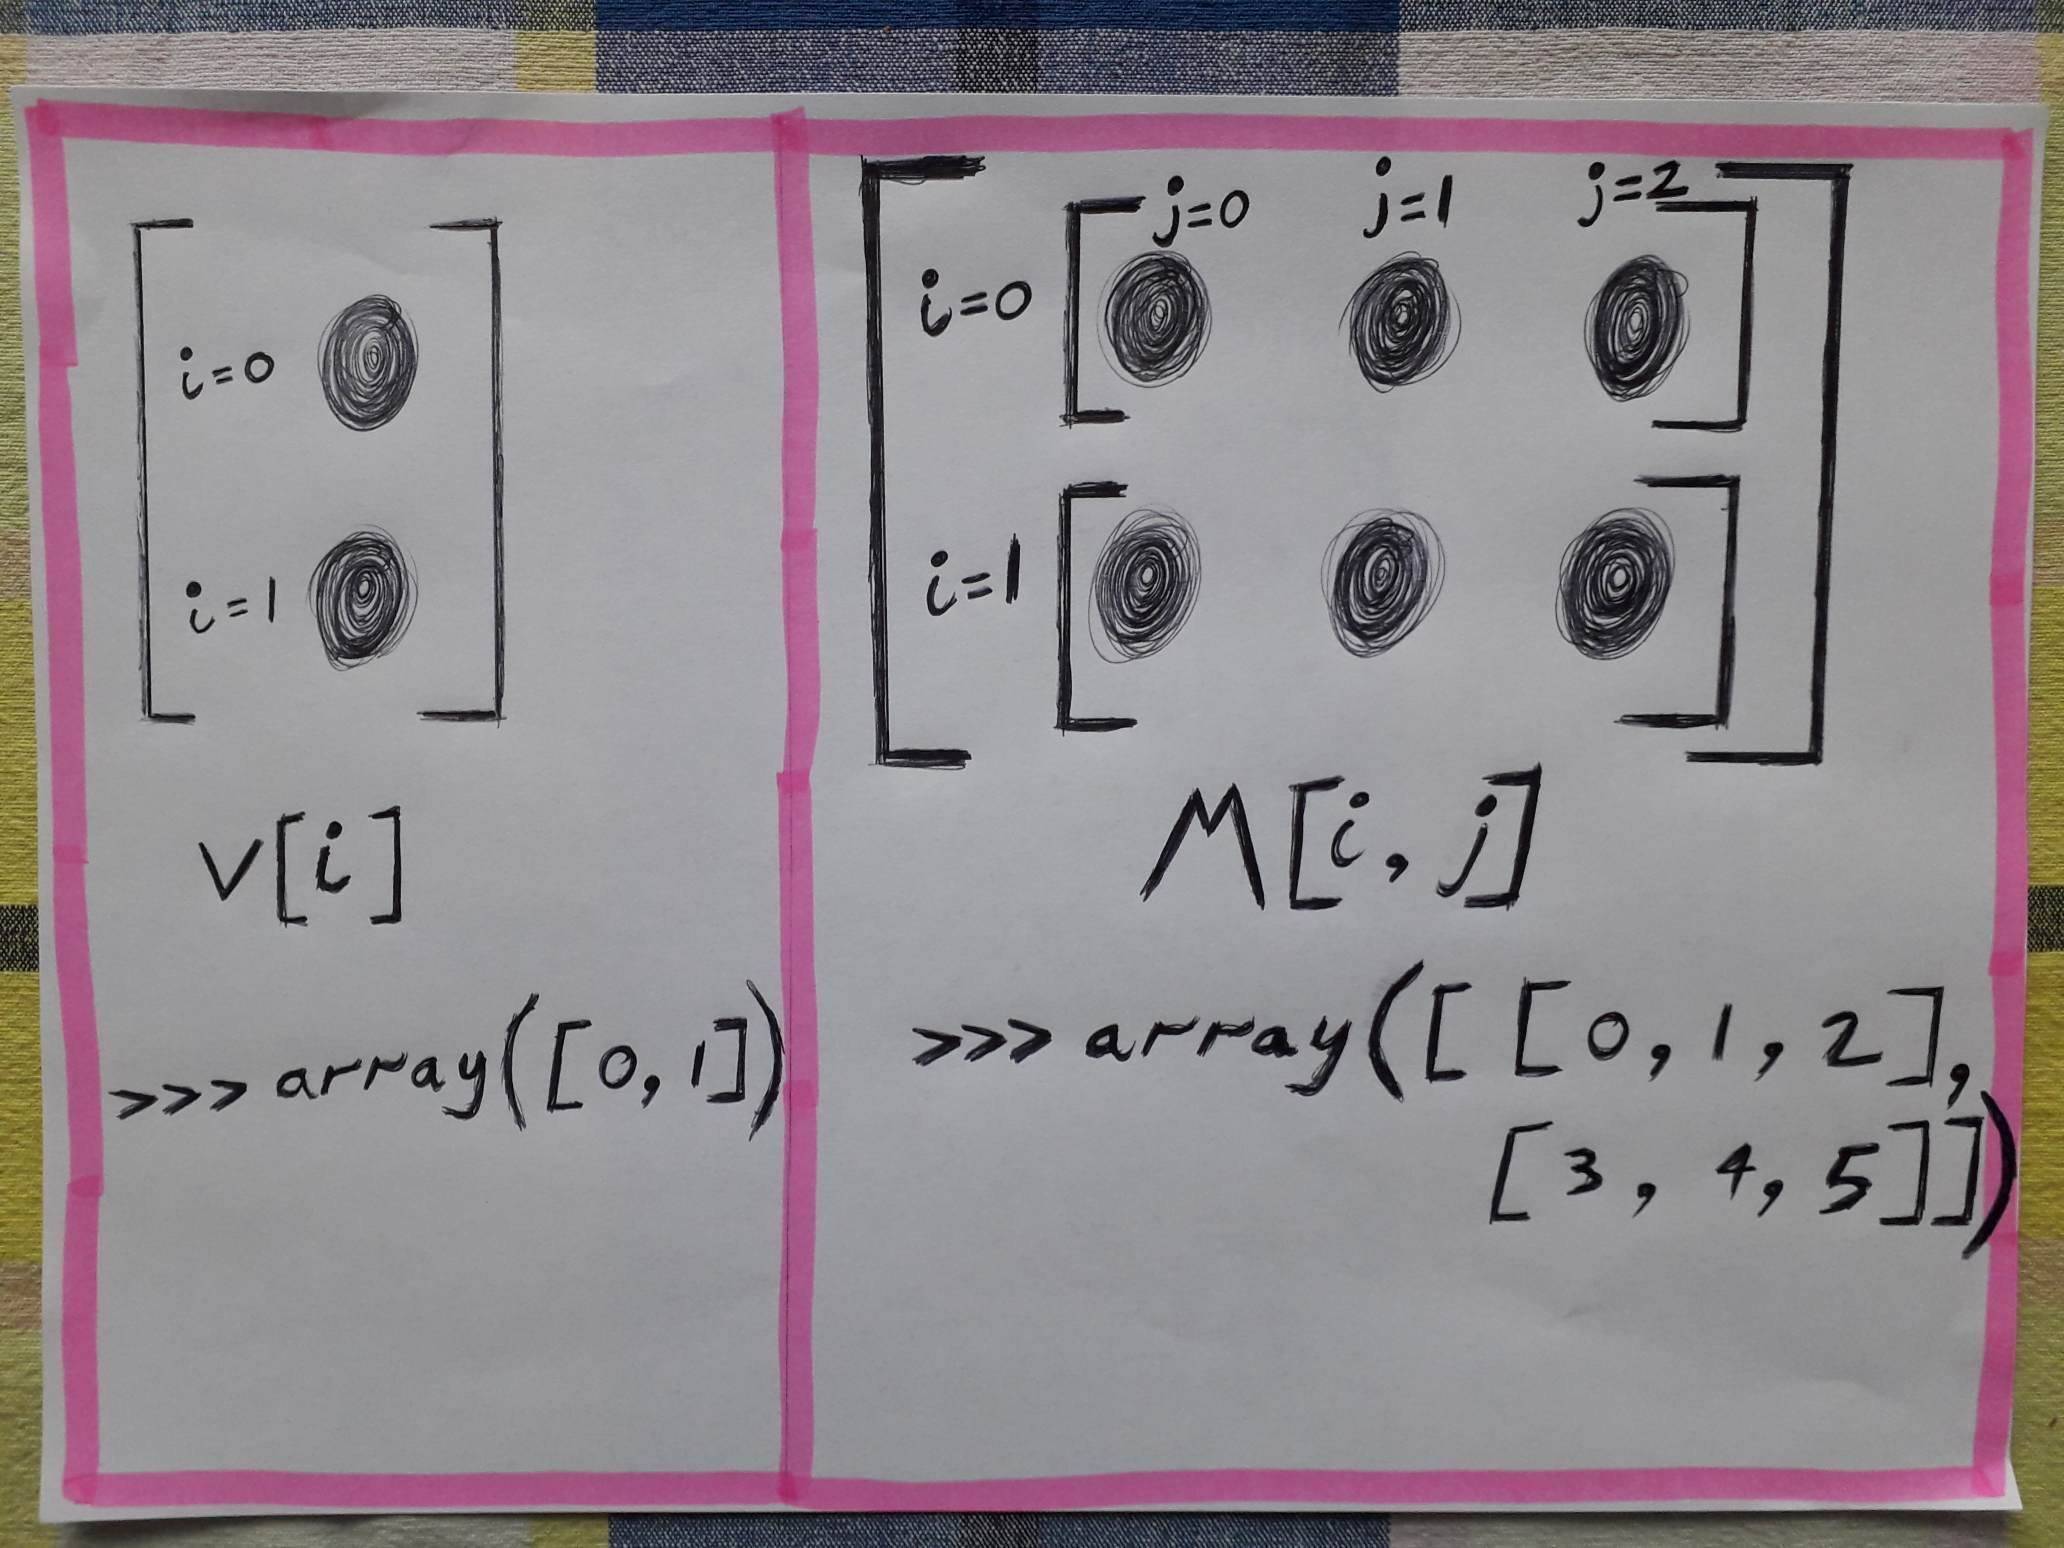
\includegraphics[width=1.00\textwidth]{./images/1d_2d_array.jpg}
\caption{
Visualization of 1D and 2D arrays, respectively.
}
\label{fig:1d_2d_array}
\end{figure}

\newpage
\begin{figure}[ht]
\centering
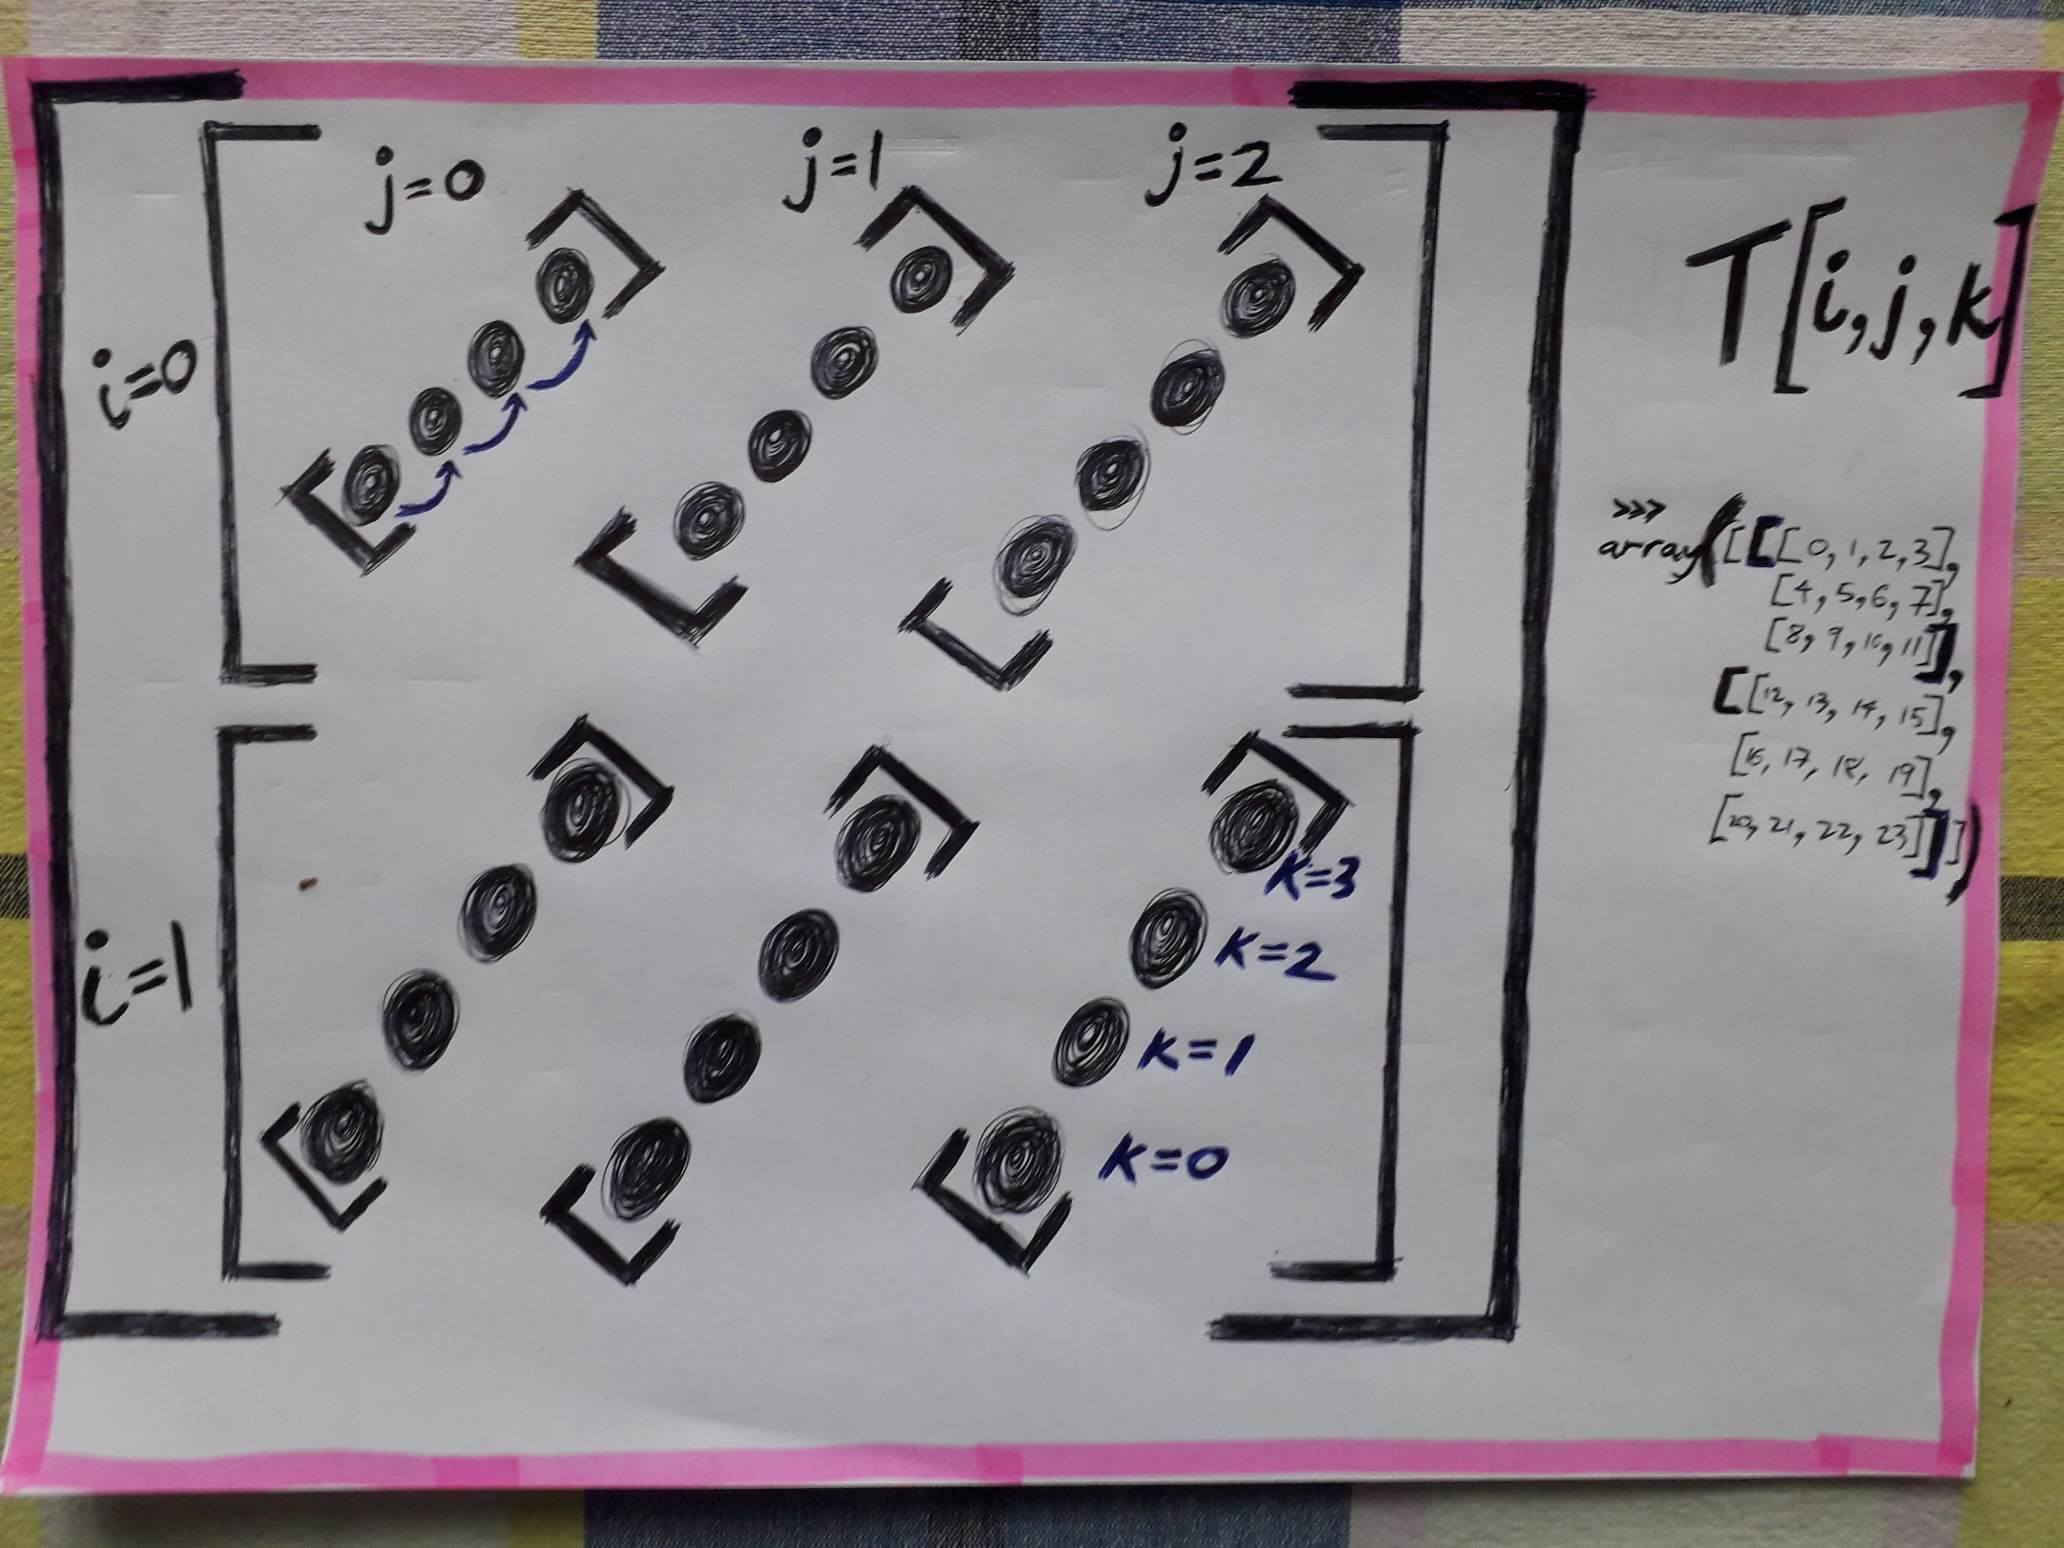
\includegraphics[width=1.00\textwidth]{./images/3d_array.jpg}
\caption{
Visualization of 3D arrays.
}
\label{fig:3d_array}
\end{figure}

\vspace{\baselineskip}
\vspace{\baselineskip}
\vspace{\baselineskip}
\vspace{\baselineskip}

\begin{figure}[ht]
\centering
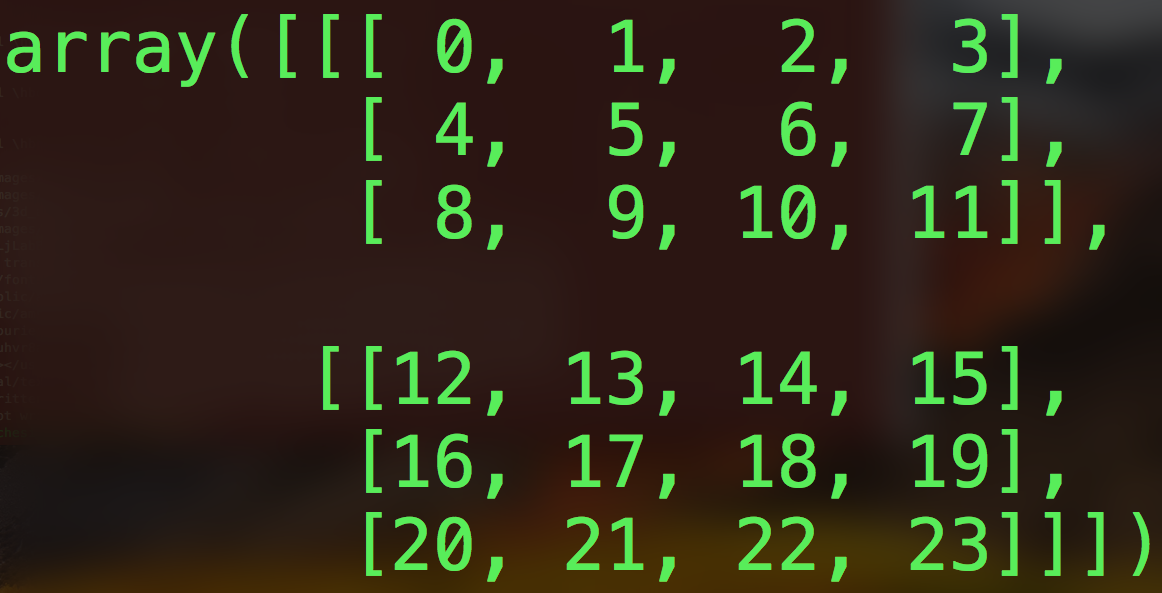
\includegraphics[width=0.65\textwidth]{./images/3d_array_print}
% \caption{
% Visualization of 3D arrays PRINTS.
% }
\label{fig:3d_array_print}
\end{figure}

\newpage
\section{PANDAS}

\vspace{\baselineskip}
\texttt{axis=0} (default) represents rows.
\newline
\texttt{axis=1} represents columns.
\newline

Read / Write:
\begin{easylist}[itemize]
\ListProperties(Style*=$\bullet$ , FinalMark={)})
& \texttt{df.to\char`_csv(\textquotesingle filename.csv\textquotesingle )} ~-- write to a CSV file.
& \texttt{pd.read\char`_csv(\textquotesingle filename.csv\textquotesingle )} ~-- read from a CSV file.
\end{easylist}
\vspace{\baselineskip}

Object Creation:
\begin{easylist}[itemize]
\ListProperties(Style*=$\bullet$ , FinalMark={)})
& \texttt{s = pd.Series([1, 2, 3, 4])} ~-- create a Series (1D).
& \texttt{s = pd.Series([1, 2, 3, 4], index=[\textquotesingle v01\textquotesingle , \textquotesingle v02\textquotesingle , \textquotesingle v03\textquotesingle , \textquotesingle v04\textquotesingle ])}
& \texttt{df = pd.DataFrame([[1,2,3],[4,5,6]])} ~-- create a DataFrame (2D).
& \texttt{df = pd.DataFrame(np.random.randn(2,3), index=[\textquotesingle v01\textquotesingle , \textquotesingle v02\textquotesingle ], columns=[\textquotesingle A\textquotesingle , \textquotesingle B\textquotesingle, \textquotesingle C\textquotesingle])}
& \texttt{df = pd.DataFrame(\{\textquotesingle A\textquotesingle :[33,22,11], \textquotesingle B\textquotesingle :[\textquotesingle baa\textquotesingle , \textquotesingle moo\textquotesingle , \textquotesingle grr\textquotesingle ]\}) }
\end{easylist}

Viewing Data:
\begin{easylist}[itemize]
\ListProperties(Style*=$\bullet$ , FinalMark={)})
& \texttt{df} ~-- top and tails the DataFrame.
& \texttt{df.head()} ~-- typical head.
& \texttt{df.tail(10)} ~-- typical tail.
& \texttt{df.index} ~-- get DataFrame index object.
& \texttt{df.columns} ~-- get DataFrame columns object.
& \texttt{df.shape} ~-- get shape of DataFrame.
& \texttt{df.size} ~-- get number of DataFrame elements.
& \texttt{df.dtypes} ~-- get the data types of the columns.
& \texttt{df.A.unique()} ~-- get the unique entries for a given column.
& \texttt{df.describe()} ~-- provides a basic statistical summary.
& \texttt{df.T} ~-- transpose the DataFrame.
& \texttt{df.to\char`_numpy()} ~-- convert DataFrame to a Numpy array.
& \texttt{df.sort\char`_index(axis=1)} ~-- sort by axis (columns).
& \texttt{df.sort\char`_index(ascending=False)} ~-- sort by axis (rows).
& \texttt{df.sort\char`_values(by=\textquotesingle B\textquotesingle)} ~-- sort by values.
\end{easylist}
\vspace{\baselineskip}

Selection:
\begin{easylist}[itemize]
\ListProperties(Style*=$\bullet$ , FinalMark={)})
& \texttt{df.A} ~-- get column A.
& \texttt{df[\textquotesingle A\textquotesingle]} ~-- select column A.
& \texttt{df[20:25]} ~-- select row slice.
& \texttt{df[\textquotesingle A\textquotesingle][20:25]} ~-- select column and row slice.
& \texttt{df.loc[25]} ~-- get row cross section.
& \texttt{df.loc["2015-09-20 10:00:30"]} ~-- as above, if the rows have names.
& \texttt{df.loc[25, [\textquotesingle A\textquotesingle,\textquotesingle B\textquotesingle]]} ~-- get row cross section for specified columns.
& \texttt{df.loc[20:25, [\textquotesingle A\textquotesingle,\textquotesingle B\textquotesingle]]}~-- select row and column slice (endpoints are \textit{included}).
& \texttt{df.loc["2015-09-20 10:00:30":"2015-09-20 10:00:40", :]}
& \texttt{df.loc[25, \textquotesingle A\textquotesingle]} ~-- get a scalar value.
& \texttt{df.at[25, \textquotesingle A\textquotesingle]} ~-- get fast access to a scalar value.
& \texttt{df.iloc[3:5, 0:2]} ~-- as above but \textbf{specifically} using integer indexing.
& \texttt{df.iloc[3:5, :]} ~-- slicing rows explicitly.
& \texttt{df.iloc[:, 0:2]} ~-- slicing columns explicitly.
& \texttt{df.iat[25, 10]} ~-- as above but \textbf{specifically} using integer indexing.
\end{easylist}
\vspace{\baselineskip}

Boolean Indexing:
\begin{easylist}[itemize]
\ListProperties(Style*=$\bullet$ , FinalMark={)})
& \texttt{df[df.A > 0]} ~-- use a column's values to select data.
& \texttt{df[df.A > 0.5 * (df.B + df.C)]} ~-- \textit{another example}.
& \texttt{df[(df.A > 50) \& (df.B > 50)]} ~-- and \textit{another example}.
& \texttt{df[df > 1.0]} ~-- select values from a DataFrame where a boolean condition is met.
& \texttt{(df > 1.0).sum()} ~-- \textit{little trick which combines techniques}.
& \texttt{df.isin([11,22,33,\textquotesingle C\textquotesingle,\textquotesingle M\textquotesingle,\textquotesingle S\textquotesingle])} ~-- take note of the \textit{isin()} method.
\end{easylist}

\newpage
Setting:
\begin{easylist}[itemize]
\ListProperties(Style*=$\bullet$ , FinalMark={)})
& \texttt{df[\textquotesingle Z\textquotesingle] = [3, 2, 6, 4]} ~-- setting a new column.
& \texttt{df[\textquotesingle Z\textquotesingle] = s} ~~-- NOTE if you use a Series, it doesn't have to be a perfect fit.
& \texttt{df.at[7, \textquotesingle C\textquotesingle] = 888 } -- set scalar values by label.
& \texttt{df.iat[7, 3] = 888 } -- set scalar values by index.
& \texttt{df.loc[:, \textquotesingle D\textquotesingle] = np.array([5] * len(df))} -- set multiple values.
& \texttt{df = df + 2 } ~-- operate on every DataFrame element.
& \texttt{df = df1 + df2 } ~-- \textit{another example}.
& \texttt{df[df < 0] = -df } ~-- can also set values using a boolean mask.
& \texttt{df[\textquotesingle A\textquotesingle] *= -1 } ~-- operate on every element in a column.
& \texttt{df[\textquotesingle A\textquotesingle] = 2 * df[\textquotesingle B\textquotesingle] + df[\textquotesingle C\textquotesingle] } ~-- \textit{another example}. Better than df.apply.
& \texttt{df.loc[3] += 55 } ~-- operate on every element in a row.
& \texttt{df.loc[3] = 2 * df.loc[4] + 55} ~-- \textit{another example}.
\end{easylist}

% \vspace{\baselineskip}
Missing Data:
\begin{easylist}[itemize]
\ListProperties(Style*=$\bullet$ , FinalMark={)})
& \texttt{df.dropna()} ~-- drop any rows with missing data.
& \texttt{df.dropna(axis=1)} ~-- drop any columns with missing data.
& \texttt{df.dropna(how=\textquotesingle any\textquotesingle)} ~-- drop row if there is \textbf{any} NaN instance (default).
& \texttt{df.dropna(how=\textquotesingle all\textquotesingle)} ~-- only drop row if \textbf{all} instances are NaN.
& \texttt{df.fillna(value=55)} ~-- fill missing data with a value.
& \texttt{df.isna()} ~-- get boolean mask where values are NaN.
% & \texttt{df.isna().sum()} ~-- \textit{little trick which combines techniques}.
\end{easylist}

Operations:
% Operations in general \textit{exclude} missing data.
\begin{easylist}[itemize]
\ListProperties(Style*=$\bullet$ , FinalMark={)})
& \texttt{df.mean()} ~-- get the mean of each column.
& \texttt{df.mean(axis=1)} ~-- get the mean of each row.
& \texttt{df.sum(), df.cumsum(), df.max()...} ~-- many different operations.
& \texttt{df.A.sum()} ~-- operate on a single column.
& \texttt{df.apply(lambda col: col.max() - col.min())} ~-- apply function    to cols.
& \texttt{df.apply(lambda row: row.A + row.B, axis=1)} ~-- apply function to rows.
\end{easylist}

Merge:
\begin{easylist}[itemize]
\ListProperties(Style*=$\bullet$ , FinalMark={)})
& \texttt{df = pd.concat([df1, df2])} ~-- concatenate DataFrames.
& \texttt{df = pd.concat([df1, df2], ignore\char`_index=True)} ~-- avoids index clash.
& \texttt{df = pd.concat([df1, df2], axis=1)} -- concatenate DataFrames side-by-side.
& \texttt{df1.append(df2.loc[5], ignore\char`_index=True)} ~-- append a new row.
& \texttt{pd.merge(df1, df2, on=\textquotesingle A\textquotesingle)} ~-- merge DataFrames with same column elements.
& \texttt{pd.merge(df1, df2, left\char`_on=\textquotesingle car\textquotesingle, right\char`_on=\textquotesingle vehicle\textquotesingle)}
~-- merge like this when columns have different names.
\end{easylist}

\vspace{\baselineskip}
Group:
\begin{easylist}[itemize]
\ListProperties(Style*=$\bullet$ , FinalMark={)})
& \texttt{df.groupby(\textquotesingle A\textquotesingle).max()}
~-- for all sets of rows with common column `A'~values,
perform function on all remaining columns.
& \texttt{df.groupby([\textquotesingle A\textquotesingle, \textquotesingle B\textquotesingle]).max()}
~-- like above, but group by both column `A'~and then column `B'.
\end{easylist}

\vspace{\baselineskip}
Time Series:
\begin{easylist}[itemize]
\ListProperties(Style*=$\bullet$ , FinalMark={)})
& \texttt{rng = pd.date\char`_range(\textquotesingle2015-09-20 10:00:00\textquotesingle,\newline .....................periods=100, freq=\textquotesingle S\textquotesingle)} -- creates datetime index.
& \texttt{rng = pd.date\char`_range(start=\textquotesingle2015-09-20 10:00:00\textquotesingle,\newline ....................end=\textquotesingle2019-07-10 17:30:00\textquotesingle, periods=100)} %~-- alternative method.
& \texttt{rng[90].year, rng[90].second} ~-- pull the specific numbers of a given date.
& \texttt{(rng[90] - rng[0]).days} ~-- calculate differences between dates.
& \texttt{df=pd.DataFrame(np.random.rand(100,3), index=rng, columns=list(\textquotesingle ABC\textquotesingle))} ~-- use datetime as a DataFrame index.
\end{easylist}

\vspace{\baselineskip}
Plotting:
\begin{easylist}[itemize]
\ListProperties(Style*=$\bullet$ , FinalMark={)})
& \texttt{df.plot()} ~-- creates graphs from DataFrame.
% & \texttt{df.A.plot()} ~-- \textit{another example}.
& \texttt{df.plot(kind=\textquotesingle scatter\textquotesingle, x=\textquotesingle A\textquotesingle, y=\textquotesingle B\textquotesingle)} ~-- \textit{another example}.
& \texttt{df.hist(bins=50)} ~-- creates histograms from DataFrame.
& \texttt{df.hist(column=\textquotesingle A\textquotesingle, bins=50)} ~-- \textit{another example}.
& \texttt{pd.plotting.scatter\char`_matrix(df[[\textquotesingle A\textquotesingle, \textquotesingle B\textquotesingle, \textquotesingle C\textquotesingle]])} ~-- scatter matrix plot.
\end{easylist}

\newpage
Miscellaneous:
\begin{easylist}[itemize]
\ListProperties(Style*=$\bullet$ , FinalMark={)})
& \texttt{df.drop(\textquotesingle A\textquotesingle, axis=1)} ~-- drop column.
& \texttt{df.drop([\textquotesingle A\textquotesingle, \textquotesingle B\textquotesingle], axis=1)} ~-- drop columns.
& \texttt{df.reindex(columns=[\textquotesingle D\textquotesingle, \textquotesingle A\textquotesingle, \textquotesingle B\textquotesingle])} ~-- select and order columns.
& \texttt{df.rename({\textquotesingle a\textquotesingle:\textquotesingle X\textquotesingle, \textquotesingle b\textquotesingle:\textquotesingle Y\textquotesingle}, axis=1)} ~-- change column names.
& \texttt{df.reset\char`_index(drop=True)} ~-- remove redundancy in indices.
\newline
& \texttt{df.nlargest(10, 'A')} ~-- returns DataFrame ordered by largest column values.
& \texttt{df.nsmallest(20, 'B')} ~-- returns DataFrame ordered by smallest column values.
& \texttt{df.A.value\char`_counts()} ~-- get frequency of column values.
\newline
& \texttt{df.sample(frac = 0.5)} ~-- get fractional random sample from DataFrame.
& \texttt{df.sample(n = 10)} ~-- get nRows random sample from DataFrame.
\end{easylist}

\newpage
\section{RESOURCES}

CPP:
\newline
\texttt{Accelerated C++} -- where I learnt.

General Python:
\newline
\texttt{http://chryswoods.com/main/courses/} -- where I learnt.
\newline
\texttt{http://www.tutorialspoint.com/python/}
\newline
\texttt{https://docs.python.org/2.7/tutorial/}

Jupyter Notebooks:
\newline
\texttt{https://www.datacamp.com/community/tutorials/tutorial-jupyter-notebook/}

NumPy:
\newline
\texttt{https://www.numpy.org/devdocs/user/quickstart.html}

Pandas:
\newline
\texttt{https://pandas.pydata.org/pandas-docs/stable/index.html}

Matplotlib:
\newline
\texttt{https://matplotlib.org/tutorials/index.html}

ML:
\newline
\texttt{Hands-on Machine Learning with Scikit-Learn, Keras, and TensorFlow}

% More / General:
% \newline
% \texttt{https://github.com/jakevdp/PythonDataScienceHandbook/}

\newpage

\end{document}